\section{Auswertung}
\label{sec:auswertung}
In den Unterkapiteln dieses Abschnittes sollen die gemessenen Werte ausgewertet werden.
\subsection{Bestimmung der Schallgeschwindigkeit}
\label{sec:schallgeschwindigkeit}
Um die Schallgeschwindigkeit im Acrylblock zu bestimmen wurde die Laufzeit des Impulses, im Impuls-Echo- Verfahren, zwischen Oberseite des 
Acrylblocks und der darunter liegenden Tischplatte bestimmt. Dazu wurde von beiden Seiten gemessen und die Schallgeschwindigkeit nach folgender
Vorschrift berechnet:
\begin{center}
    $c_{Acryl}=\frac{H}{t_1}+\frac{H}{t_2}$\\
\end{center}
Mit $H$ der mittels eies Messschiebers bestimmten Höhe des Acrylblocks und $t_1$, $t_2$ den Laufzeiten des Ultraschallimpulses.
\begin{center}
    $H=(79.5\pm 0.1)\si[]{mm} $\\
    $t_1=(59.2)\si[]{\mu s}$\\
    $t_2=(59.2)\si[]{\mu s}$\\ 
    $\Rightarrow$ $c_{Acryl}=(2685.8\pm3.4)\si[]{\frac{m}{s}}$
\end{center}

\subsection{Bestimmung der Positionen der Fehlstellen}
\label{sec:fehlstellen}
Über \autoref{eq:weg} können nun sofort die Positionen der Fehlstellen berechnet werden. In der nachstehenden Tabelle \autoref{tab:pos} sind die berechneten 
Positionen aufgführt. Im Diagram \autoref{fig:acrylblock} ist eine schematische Darstellung des Acrylblocks zu sehen,
Die X-Achse bildet dabei die untere Kante des Acrylblocks und die Y-Achse die linke Seite. Die Schwarzen Punkte 
deuten die Mittelpunkte der Fehlstellen an, während die roten Kreuze die bei der Messung von oben und die grünen
Kreuze auf die bei der Messung von unten entsandenen Messwerte zeigen. 
\begin{table}
  
    \centering
    
    \caption{Laufzeiten und errechnete Positionen}
    \label{tab:pos}
    \sisetup{table-format=1.2}
    \begin{tabular}{S[table-format=3.2] S S S S S [table-format=3.2]}
      \toprule
      {Fehlstelle Nr} & {Position [mm]} &{Laufzeit $t_1$ [$\mu s$]}&  {Position [mm]} & {Laufzeit $t_2$ [$\mu s$]}\\
      \midrule
      1 & {$$18.801\pm 0.024$$ }&{$$14.0$$  } & {$$60.830\pm 0.080$$} & {$$45.3$$} \\
      2 & {$$20.412\pm 0.026$$ }&{$$15.2$$  } & {$$59.220\pm 0.070$$} & {$$44.1$$} \\
      3 & {$$60.700\pm 0.080$$ }&{$$45.2$$  } & {$$14.369\pm 0.018$$} & {$$10.7$$} \\
      4 & {$$53.310\pm 0.070$$ }&{$$39.7$$  } & {$$22.561\pm 0.028$$} & {$$16.8$$} \\
      5 & {$$46.060\pm 0.060$$ }&{$$34.3$$  } & {$$28.201\pm 0.035$$} & {$$21.0$$} \\
      6 & {$$38.540\pm 0.050$$ }&{$$28.7$$  } & {$$39.080\pm 0.050$$} & {$$29.1$$} \\
      7 & {$$30.750\pm 0.040$$ }&{$$22.9$$  } & {$$47.140\pm 0.060$$} & {$$35.1$$} \\
      8 & {$$23.098\pm 0.029$$ }&{$$17.2$$  } & {$$55.060\pm 0.070$$} & {$$41.0$$} \\
      9 & {$$15.041\pm 0.019$$ }&{$$11.2$$  } & {$$62.710\pm 0.080$$} & {$$46.7$$} \\
      10& {$$7.3860\pm 0.009$$ }&{$$ 5.5$$  } & {verdeckt           } & {verdeckt} \\
      11& {$$54.660\pm 0.070$$ }&{$$40.7$$  } & {$$16.383\pm 0.021$$} & {$$46.7$$} \\

      \bottomrule
    
    \end{tabular}
  \end{table}
  \begin{figure}
    \centering
    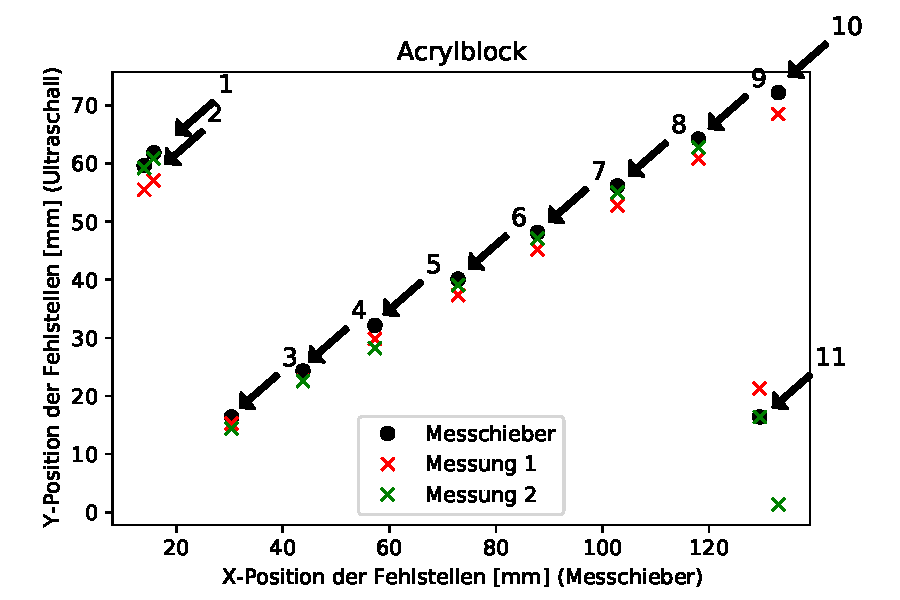
\includegraphics{acrylblock.pdf}
    \caption{Position von Fehlstellen im Acrylblock}
    \label{fig:acrylblock}
  \end{figure}
  \pagebreak
  
  \subsection{Vermessung eines Augenmodells}
  \label{sec:auge}

  \begin{figure}[h]
    \label{fig:auge}
    \centering
    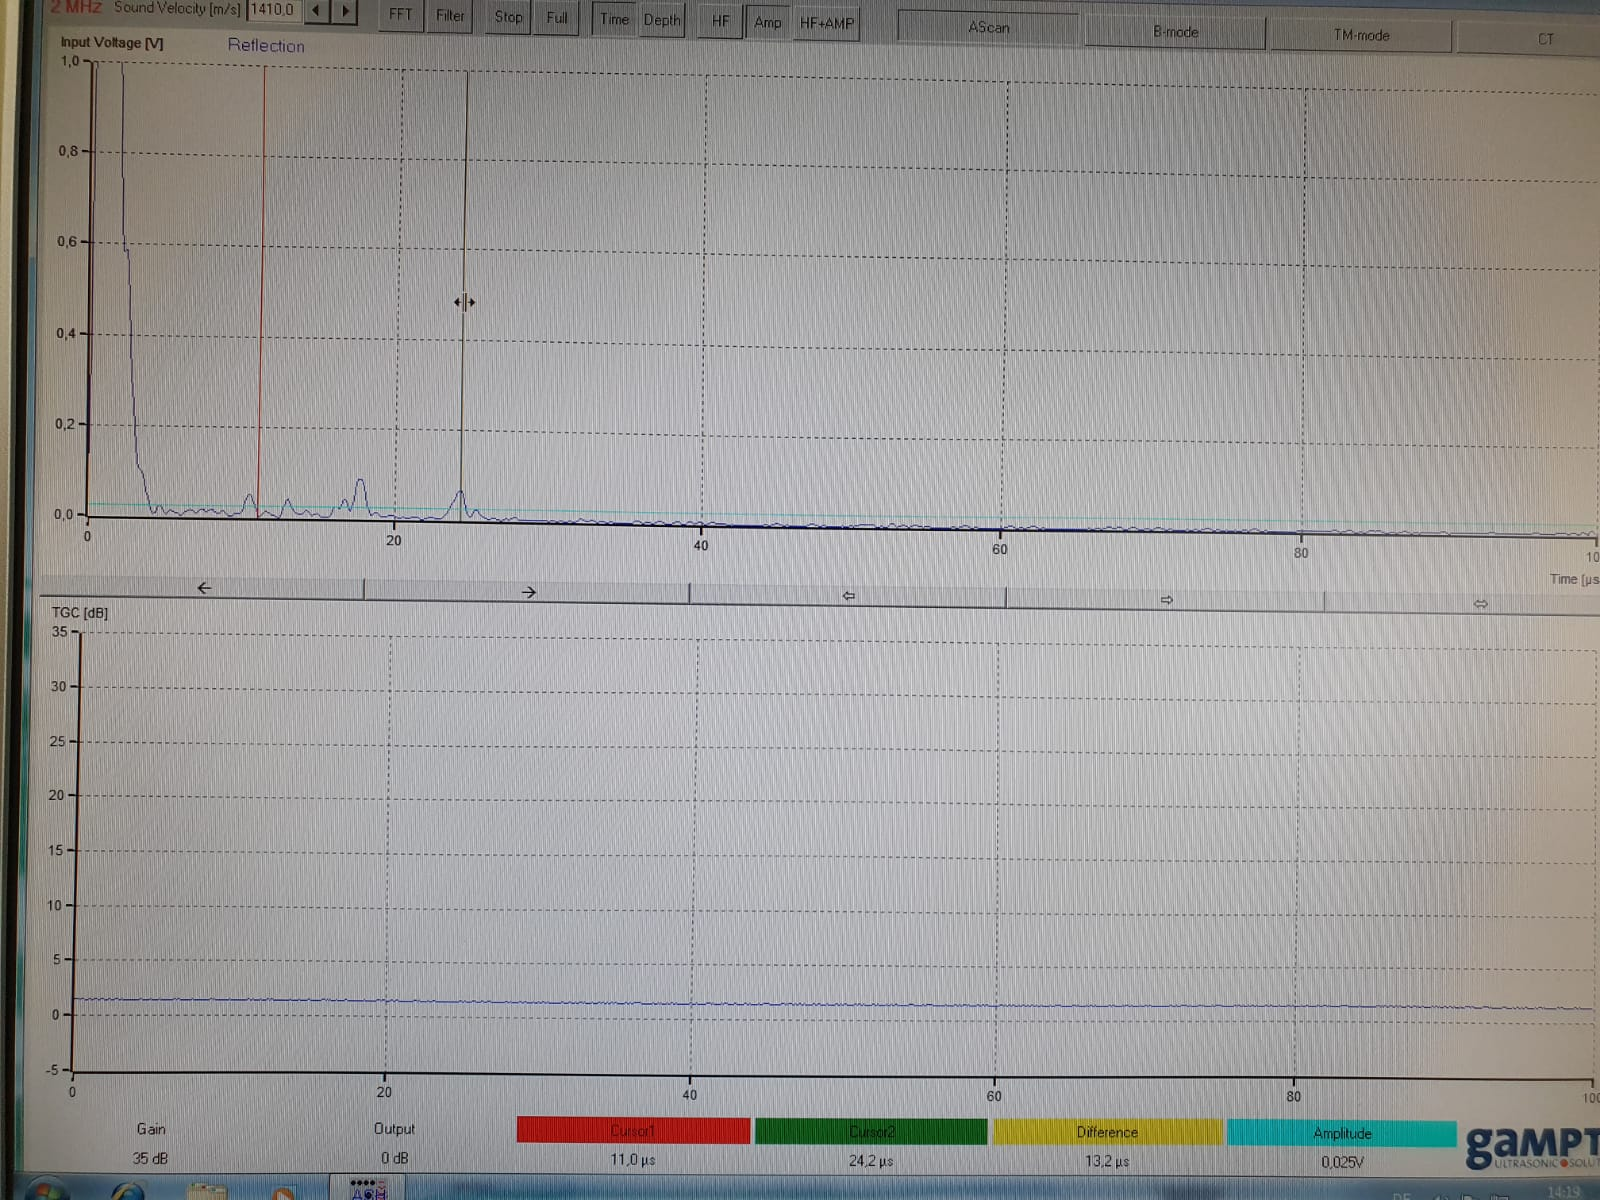
\includegraphics[width=10cm]{Auge}
    \caption{U-T-Diagramm eines Augenmodells}
\end{figure}
In \autoref{fig:augee} sind vier recht nah beieinander gelegene Peaks zu sehen, dabei handelt es sich sehr wahrscheinlich um:\\
 1. Die Hornhaut\\
 2. Die vordere Augenkammer\\
 3. Die Linse\\
 4. Den Glaskörper\\
 bzw. die jweilige Grenzfläche zum davor gelegenen Teil. Ein Peak der die Netzhaut repräsentieren würde ist leider nicht zu erkennen oder verschwindet 
 im Untergrund.   